\documentclass[journal,12pt,twocolumn]{IEEEtran}
\usepackage{graphicx}
\usepackage[margin=0.5in]{geometry}
\usepackage[cmex10]{amsmath}
\usepackage{array}
\usepackage{booktabs}
\usepackage{mathtools}
\usepackage{hyperref}


\title{\textbf{FPGA assignment}}
\author{kanekal kousar}
\date{September 2022}


\begin{document}
\maketitle

\begin{enumerate}
    \item \textbf{Abstract}:Through this manual, we learn how to display sum of two numbers on LCD using fpga
Let this pin be V cc 
    \item \textbf{components}
\end{enumerate}
     \begin{tabular}{ |p{3cm}|p{1.5cm}|p{1.5cm}| }
 \hline
 \setlength{\tabcolsep}{3pt}
components & values & quantity \\
\hline
 Vaman Board &   - & 1\\
 LCD &16x2 & 1\\
 bread board  &-& 1\\
 jump wires&  - & 20\\
 \hline
\end{tabular}
\begin{center}
    TABLE I
\end{center}

\begin{enumerate}
    \item[--] \textbf{step 1}:-Connect the 5V pin of the Vaman to an extreme pin of the Breadboard
Let this pin be V cc 
    \item[--] \textbf{step 2}:-Connect the GND pin of the Vaman to the opposite extreme pin of the Breadboard.
     \item[--] \textbf{step 3}:-plug the LCD in fig.7 to breadboard
    \item[--] \textbf{step 4}:-make the connections of vaman board and LCD according to tableII
   
\end{enumerate}


\begin{center}
    TABLE II :Vaman to LCD connections
\end{center}
 \begin{tabular}{ |p{1.5cm}|p{1.5cm}|p{1.5cm}|p{1.5cm}| }
 \hline
 \setlength{\tabcolsep}{3pt}
Pygmy & LCD pins & LCD pin label & LCD pin Description\\
\hline
 GND & 1& GND & \\
 \hline
 5V & 2 & Vcc &\\
 \hline
 GND & 3 & Vee & Contrast\\
 \hline
 10 & 4 & RS & Register Select\\
 \hline
 GND & 5 & R/W & read/write\\
 \hline
 9 & 6 & EN &Enable\\
 \hline
 14 & 11 & DB4 & Serial connection\\
 \hline
 13 & 12 & DB5 & Serial connection\\
 \hline
 12 & 13 & DB6 & Serial connection\\
 \hline
 11 & 14 & DB7 & Serial connection\\
 \hline
 5V & 15 & LED+ & Backlight\\
 \hline
 GND & 16 & LED- & Backlight\\
 \hline
\end{tabular}



\begin{figure}[h!]
\vspace{7cm}
\centering
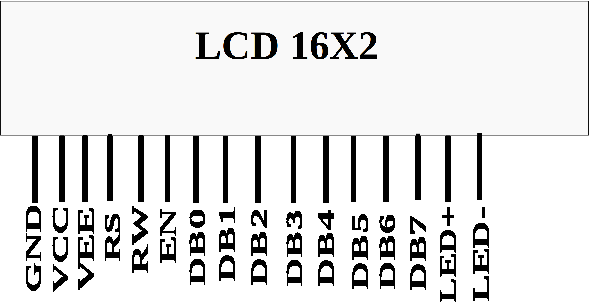
\includegraphics[scale=0.5]{figs/lcd.png}   \\
\centering
\caption{LCD 16X2}
\end{figure}


\newpage \section*{CODE}
-After connection write the following verilog code
\begin{enumerate}
\item[]\hspace{-2cm}\url{https://github.com/kkousar/KOUSAR_FWC/tree/main/fpga/code}
\end{enumerate}



   


\end{document}





